%% Based on a TeXnicCenter-Template by Tino Weinkauf.
%%%%%%%%%%%%%%%%%%%%%%%%%%%%%%%%%%%%%%%%%%%%%%%%%%%%%%%%%%%%%

%%%%%%%%%%%%%%%%%%%%%%%%%%%%%%%%%%%%%%%%%%%%%%%%%%%%%%%%%%%%%
%% HEADER
%%%%%%%%%%%%%%%%%%%%%%%%%%%%%%%%%%%%%%%%%%%%%%%%%%%%%%%%%%%%%
\documentclass[a4paper,10pt]{article}

% Alternative Options:
%	Paper Size: a4paper / a5paper / b5paper / letterpaper / legalpaper / executivepaper
% Duplex: oneside / twoside
% Base Font Size: 10pt / 11pt / 12pt

\usepackage{fontspec}
\usepackage{polyglossia}
\setmainlanguage{spanish}


%% Packages for Graphics & Figures %%%%%%%%%%%%%%%%%%%%%%%%%%
\usepackage{graphicx} %%For loading graphic files
%\usepackage{subfig} %%Subfigures inside a figure
%\usepackage{pst-all} %%PSTricks - not useable with pdfLaTeX

%% Please note:
%% Images can be included using \includegraphics{Dateiname}
%% resp. using the dialog in the Insert menu.
%% 
%% The mode "LaTeX => PDF" allows the following formats:
%%   .jpg  .png  .pdf  .mps
%% 
%% The modes "LaTeX => DVI", "LaTeX => PS" und "LaTeX => PS => PDF"
%% allow the following formats:
%%   .eps  .ps  .bmp  .pict  .pntg


%% Math Packages %%%%%%%%%%%%%%%%%%%%%%%%%%%%%%%%%%%%%%%%%%%%
\usepackage{amsmath}
\usepackage{amsthm}
\usepackage{amsfonts}



%% Line Spacing %%%%%%%%%%%%%%%%%%%%%%%%%%%%%%%%%%%%%%%%%%%%%
%\usepackage{setspace}
%\singlespacing        %% 1-spacing (default)
%\onehalfspacing       %% 1,5-spacing
%\doublespacing        %% 2-spacing

\usepackage{fancyhdr}
\setlength{\headheight}{13pt} 

%% Other Packages %%%%%%%%%%%%%%%%%%%%%%%%%%%%%%%%%%%%%%%%%%%
\usepackage{a4wide} %%Smaller margins = more text per page.
%\usepackage{fancyhdr} %%Fancy headings
%\usepackage{longtable} %%For tables, that exceed one page


%%%%%%%%%%%%%%%%%%%%%%%%%%%%%%%%%%%%%%%%%%%%%%%%%%%%%%%%%%%%%
%% Remarks
%%%%%%%%%%%%%%%%%%%%%%%%%%%%%%%%%%%%%%%%%%%%%%%%%%%%%%%%%%%%%
%
% TODO:
% 1. Edit the used packages and their options (see above).
% 2. If you want, add a BibTeX-File to the project
%    (e.g., 'literature.bib').
% 3. Happy TeXing!
%
%%%%%%%%%%%%%%%%%%%%%%%%%%%%%%%%%%%%%%%%%%%%%%%%%%%%%%%%%%%%%

%%%%%%%%%%%%%%%%%%%%%%%%%%%%%%%%%%%%%%%%%%%%%%%%%%%%%%%%%%%%%
%% Options / Modifications
%%%%%%%%%%%%%%%%%%%%%%%%%%%%%%%%%%%%%%%%%%%%%%%%%%%%%%%%%%%%%

%\input{options} %You need a file 'options.tex' for this
%% ==> TeXnicCenter supplies some possible option files
%% ==> with its templates (File | New from Template...).



%%%%%%%%%%%%%%%%%%%%%%%%%%%%%%%%%%%%%%%%%%%%%%%%%%%%%%%%%%%%%
%% DOCUMENT
%%%%%%%%%%%%%%%%%%%%%%%%%%%%%%%%%%%%%%%%%%%%%%%%%%%%%%%%%%%%%
\begin{document}
%
% Hago que en la cabecera de página se muestre a la derecha la sección,
% y en el pie, en número de página a la derecha:
%
\pagestyle{fancy}
\renewcommand{\sectionmark}[1]{\markboth{}{\thesection\ \ #1}}
\lhead{}
\chead{}
\rhead{\rightmark}
\lfoot{}
\cfoot{}
\rfoot{\thepage}

%% Title Page %%%%%%%%%%%%%%%%%%%%%%%%%%%%%%%%%%%%%%%%%%%%%%%
%% ==> Write your text here or include other files.

%
% Carátula:
%

\author{Firstname Lastname}
%\date{} %%If commented, the current date is used.

\begin{titlepage}

\thispagestyle{empty}
\begin{center}

\includegraphics[scale=0.2]{imagenes/FIUBA_ALTA.jpg}\\
\large{\textsc{Universidad de Buenos Aires}}\\
\large{\textsc{Facultad De Ingeniería}}\\
\small{Año 2015 - 2\textsuperscript{do} Cuatrimestre}\\
\vspace{1cm}
\Large{\underline{\textsc{Taller de Desarrollo de Proyectos (75.45)}}}
\end{center}



%% The simple version:
\title{Sistema de Consultas Médicas Dr. Me.}

\begin{center}
\Large{\textit{\bf{Sistema de Consultas Médicas}}}\\
\Large{\textit{\bf{Dr. Me}}}\\
\textit{\bf{Modelado del sistema}}
\end{center}

\vspace{1cm}

\raggedright{\Large{\textit{\bf{Integrantes}}}}

\vspace{0.5cm}

\begin{center}
  Julián Scialabba,	\textit{P. 00.000},	\textit{julian.scialabba@gmail.com}		\\
  Facundo Rossi,		\textit{P. 00.000},	\textit{frossi85@gmail.com}		\\
  Débora Martin,		\textit{P. 00.000},	\textit{debbie1new.world@gmail.com}	\\
  Matías Manzano,			\textit{P. 00.000},	\textit{matsebman@gmail.com}		\\
  Ariel Barreiro,		\textit{P. 00.000},	\textit{damian168@gmail.com}		\\
  Sebastian Rial,			\textit{P. 00.000},	\textit{aberrei@gmail.com}		\\
\end{center}

\end{titlepage}

%
% Hago que las páginas se comiencen a contar a partir de aquí:
%

\setcounter{page}{1}

%
% Pongo el índice en una página aparte:
%

\newpage
\tableofcontents

\newpage
\section{Objetivo}
El objetivo de este proyecto es realizar un sistema que permita a cualquier persona registrada en el mismo, obtener 
un simple diagn\'ostico aproximado a partir de los s\'intomas que tal persona presenta, y darle opciones de obtener un turno m\'edico acorde en forma autom\'atica y de acuerdo a sus preferencias.

\section{Descripci\'on}
Sistema de de turnos con derivador a especialista con un listado de posibles enfermedades relacionadas a los síntomas ingresados, por proximidad y preferencias de carga de los mismos.
Muchas veces el médico clínico (primer encuentro con la medicina ante un problema) es una suerte de derivador a especialistas y/o a la realizaci\'on de estudios. 
Esta primera consulta puede ser reemplazable por un sistema online con opciones de diagnóstico desplegables a partir de las cuales y con una base de datos con conocimientos de medicina, podría indicar el especialista a consultar sin la necesidad de ir un clinico. Esta aplicación detecta el problema que podría estar padeciendo el paciente, y registra turnos en base a preferencias del usuario, para especialistas y estudios. Esto podría atacar en principio los casos más relevantes, dejando al medico clinico con los casos que caen fuera de su alcance. Luego se puede ir actualizando su base de datos con circuitos de reconocimiento de patologías más complejas pero con síntomas claramente identificables. 
El sistema sacaría turnos de acuerdo con la obra social que maneja el usuario, preferencias, cercanía, médico de cabecera, proximidad de fechas, urgencias, etc. unificando gran parte del proceso de turnos en una única interfaz.


\section{Funcionalidades}
\begin{itemize}
	\item{Consulta online de turnos en base a síntomas prefijados (Derivador a especialista).}
	\item{Obtención de turnos para especialistas:}
	\begin{itemize}
		\item{Por zona}
		\item{Por menor tiempo de espera}
		\item{Por medico que le interesa ir}
		\item{Por tipo de obra social}
		\item{Por sanatorio}
		\item{Por emergencia (urgencias, guardia)}
	\end{itemize}
	\item{Cancelación de turnos por parte de médico y paciente.}
	\item{Movimiento de turnos.}
	\item{Retroalimentación para mejorar la calidad del diagnóstico en base a la experiencia de los usuarios con la herramienta.}
	\item{Ficha médica online del paciente (Histórico) para que el especialista pueda diagnosticar}
	\item{Notificaciones para turnos en el mismo dia y el día anterior.}
	\item{Posibilidad de alertar a pacientes del dia de un especialista una demora general en la atención.}
	\item{Utilizando geoposicionamiento para detectar si es probable que llegue a tiempo al turno, caso contrario poder avisar cancelación.}
	\item{Seguimiento del paciente con alarmas/notificaciones de controles rutinarios. De estilo: tenes que ir al dentistas ya que la última vez fue hace 9 meses.}
\end{itemize}
\begin{center}
	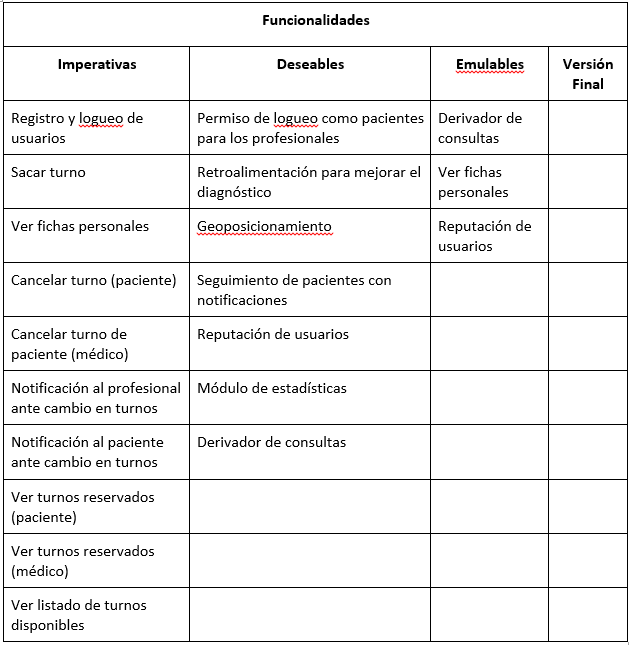
\includegraphics[scale=0.65]{imagenes/tablaFuncionalidad.png}
\end{center}

\newpage
\section{Casos de Uso}

\subsection{Listado de casos de uso}

\begin{enumerate}
	\item{Consultar Turnos: El paciente consulta los turnos que tiene asignados. Puede ver todos los turnos
	asignados simultaneamente, y puede consultar cada uno por separado, para obtener informaci�n mas espec�fica }
	\item{Pedir Turno: El paciente solicita un turno. Puede solicitarlo directamente eligiendo la especialidad o puede seguir la sugerencia del sistema ingresando sus s�ntomas.}
	\item{Cancelar Turno: Tanto el paciente como el profesiona pueden cancelar sus turnos individualmente. Al hacerlo se le enviar� una notificaci�n a la contraparte}
	\item{Visualizar Historial de Turnos: El paciente visualiza su historial de turnos, donde puede ver no solamente los turnos asignados actualmetne sino tambi�n los turnos cancelados y aquellos que ya fueron finalizados, y el resultado de
	la consulta}
	\item{Administrar Disponibilidad: El profesional decide la disponibilidad de turnos que desea otorgar, eligiendo horarios y fechas en los cuales esta disponible para atender. Hay un m�ximo sobre las fechas que puede elegir.}
	\item{Consultar ficha de paciente: El profesional consulta la ficha del paciente donde puede obtener informaci�n personal del mismo (nombre, DNI, fecha nacimiento, etc) y puede ver su historial cl�nico.}
	\item{Finalizar Turno: El profesional ha atendido al paciente, y ya puede completar el turno con el resultado del mismo. La informaci�n se agrega luego al historial cl�nico del paciente.}
	\item{Modificar Especialidades: El profesional modifica las especialidades con que va a trabajar, impactando esta modificaci�n en los turnos que los pacientes pueden solicitar.}
\end{enumerate}

\subsection{Especificaci�n de Casos de Uso}

\begin{center}
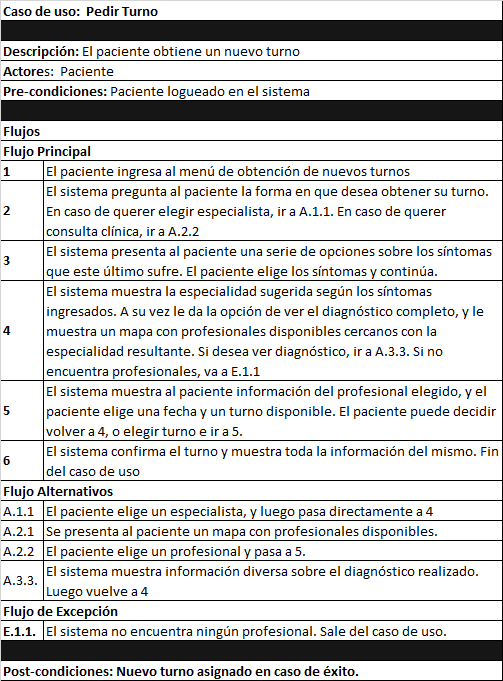
\includegraphics[scale=1]{imagenes/casosDeUso/PedirTurno.png}\\
\vspace{1cm}
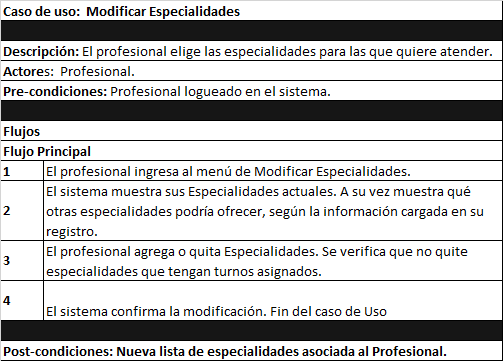
\includegraphics[scale=1]{imagenes/casosDeUso/ModificarEspecialidades.png}\\
\vspace{1cm}
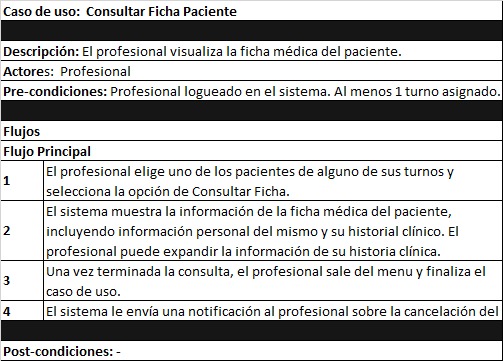
\includegraphics[scale=1]{imagenes/casosDeUso/ConsultarFichaPaciente.png}\\
\vspace{1cm}
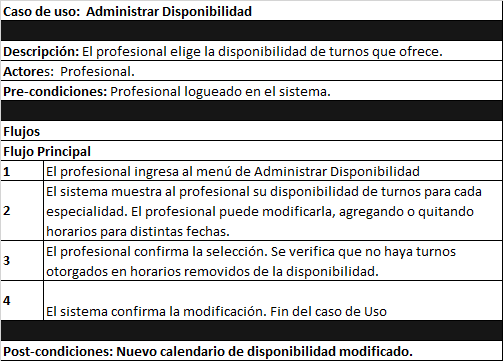
\includegraphics[scale=1]{imagenes/casosDeUso/AdministrarDisponibilidad.png}\\
\vspace{1cm}
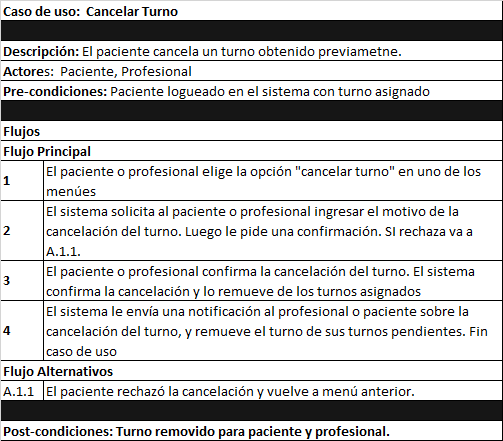
\includegraphics[scale=1]{imagenes/casosDeUso/CancelarTurno.png}\\
\vspace{1cm}
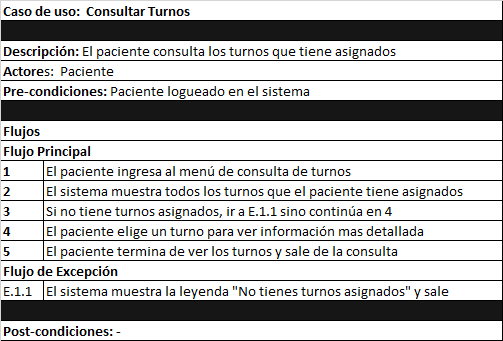
\includegraphics[scale=1]{imagenes/casosDeUso/ConsultarTurnos.png}\\
\vspace{1cm}
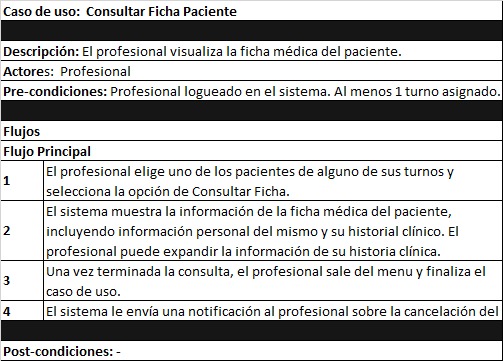
\includegraphics[scale=1]{imagenes/casosDeUso/ConsultarFichaPaciente.png}\\
\end{center}

\newpage
\subsection{Diagrama de Casos de Uso}
\begin{center}
	\includegraphics[scale=0.4]{imagenes/CasosdeUso.png}
\end{center}

\newpage
\section{Implementaci�n y Tecnolog�a Utilizada}
El proyecto se realiza por completo mediante software, su implementaci�n no incluye el funcionamiento de ninguna 
pieza espec�fica de hardware.
A continuaci�n se presenta una breve descripci�n de las tecnolog�as de software utilizadas.

Front-End: Nativescript 1.6.0. Framework multiplataforma que permite compilar la aplicaci�n tanto para Android como 
iOS y Windows Phone.\\
Back-End:\\ 
Datos:\\
Lenguajes:\\

\end{document}

